\section{Materials and methods}

% En estos capítulos, es necesario describir:
% •	los aspectos más relevantes del diseño y desarrollo del trabajo
% •	la metodología elegida para realizar este desarrollo, describiendo las alternativas posibles, las decisiones tomadas, y los criterios utilizados para tomar estas decisiones.
% •	descripción de los productos obtenidos.
 
% La estructuración de los capítulos puede variar en función del tipo de trabajo.  
 
% En caso de que proceda, se incluirá un apartado de “Valoración económica del trabajo”. Este apartado indicará los gastos asociados al desarrollo y mantenimiento del trabajo, así como los beneficios económicos obtenidos y un análisis final sobre la viabilidad del producto.

\subsection{Data Acquisition}

\subsubsection{Mouse MSI-1 and MSI-1's RMM1}

\href{https://www.uniprot.org/}{\texttt{Uniprot}'s database} was consulted for the structure of the mouse MSI-1 protein (see \textbf{Figure \ref{fig:Q61474uniprot}}). Unfortunately, there was no NMR crystal structure for the complete protein: the only available complete structure was \texttt{AlphaFold}'s prediction of the structure (see \textbf{Figure \ref{fig:3DMSI}}). Said structure had low confidence in the aminoacid sequence not corresponding to the RRMs. Therefore, the crystal structure of MSI-1's RRM1 (see \textbf{Figure \ref{fig:3DRRM1}}) was to be employed instead for the docking simulations.

\begin{figure}[htbp!]
    \centering
    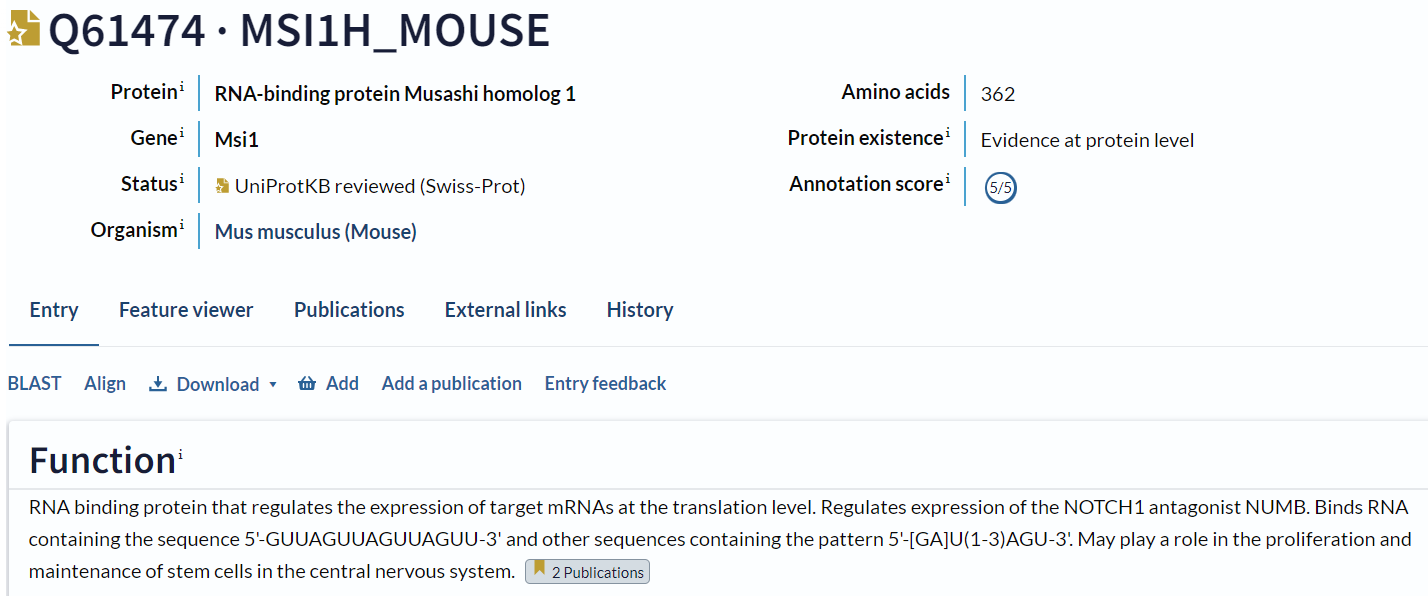
\includegraphics[width=\linewidth]{assets/Q61474_uniprot_entry.png}
    \caption[\href{https://www.uniprot.org/uniprotkb/Q61474/entry}{Uniprot entry Q61474} corresponding to the mouse MSI-1.]{\href{https://www.uniprot.org/uniprotkb/Q61474/entry}{Uniprot entry Q61474} corresponding to the mouse MSI-1 (as seen on 08/01/2023).}
    \label{fig:Q61474uniprot}
\end{figure}

The crystal NMR structure was downloaded as a \texttt{.pdb} file.

\subsubsection{Fatty acids}

The fatty acids to be employed down the line in the docking simulations were retrieved from their respective \href{https://www.chemspider.com/}{\texttt{Chemspider}} entries. The fatty acids downloaded were:

\begin{itemize}
    \item\href{https://www.chemspider.com/Chemical-Structure.392692.html}{arachidonic acid}
    \item\href{https://www.chemspider.com/Chemical-Structure.4444105.html}{linoleic acid}
    \item\href{https://www.chemspider.com/Chemical-Structure.393217.html}{oleic acid}
    \item\href{https://www.chemspider.com/Chemical-Structure.960.html}{palmitic acid}
    \item\href{https://www.chemspider.com/Chemical-Structure.5091.html}{stearic acid}
\end{itemize}

The molecules are shown in \textbf{Figure \ref{fig:fatty_acids}}.

\begin{figure}[htbp!]
    \centering
    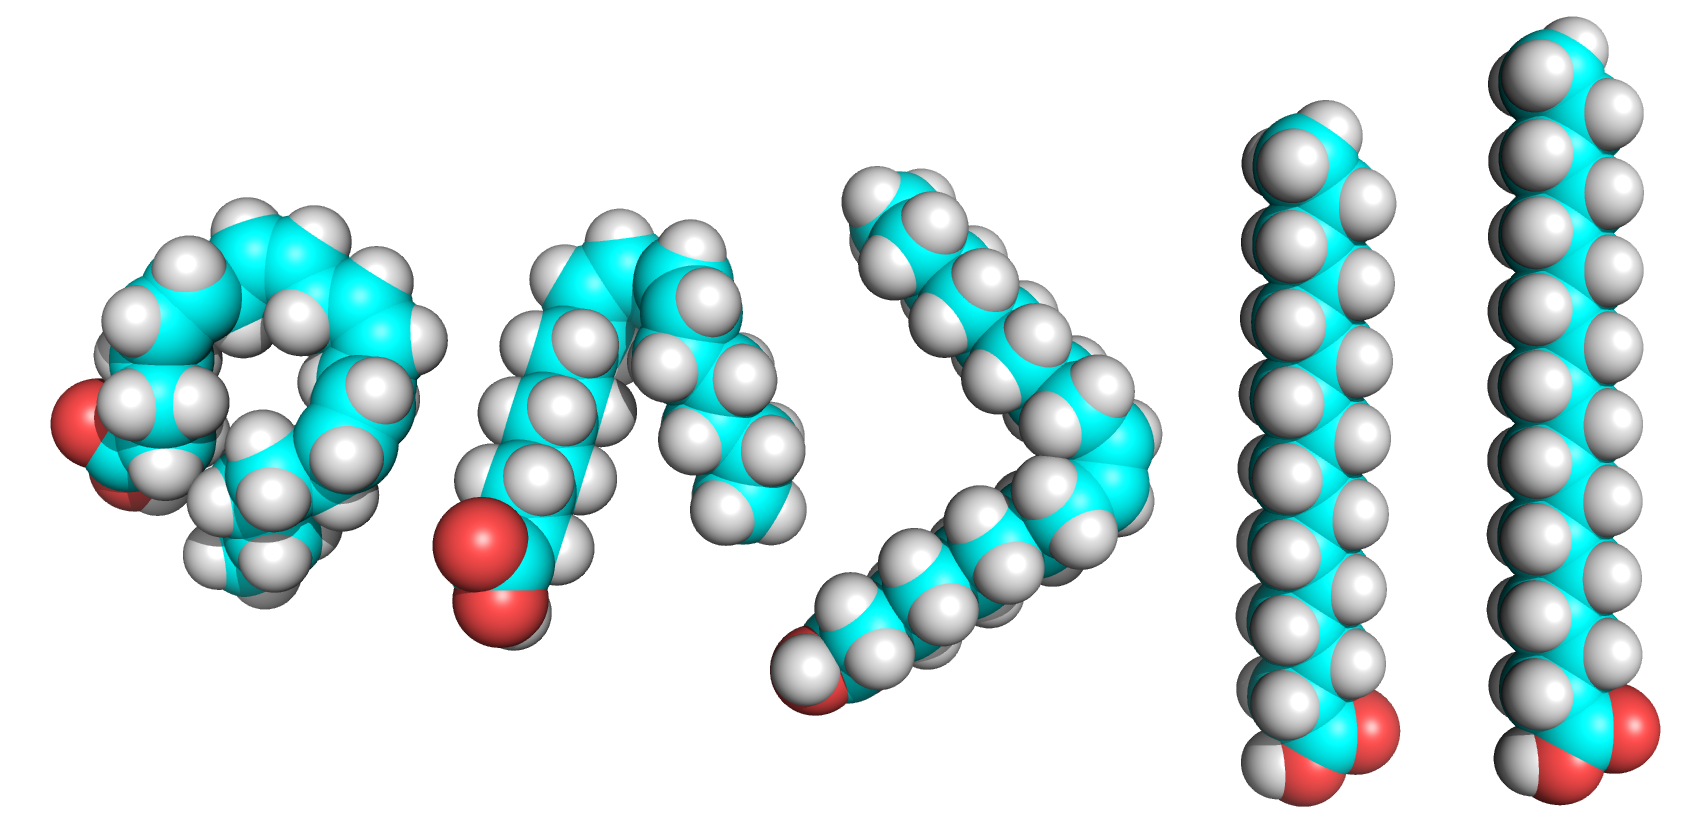
\includegraphics[width=0.75\linewidth]{assets/fatty_acids.png}
    \caption[3D structure of the fatty acids to be employed.]{3D structure of the fatty acids to be employed. From left to right: arachidonic acid, linoleic acid, oleic acid, palmitic acid and stearic acid. Colors represent the atoms present in the structures: cyan is Carbon, red is Oxygen and white is Hydrogen. Visualized through \href{https://pymol.org/2/}{\texttt{Pymol}}.}
    \label{fig:fatty_acids}
\end{figure}

The molecules' 3D structures were downloaded as \texttt{.mol} files. 

\subsection{Generation of 3D RNA molecule structures}

The raw RNA sequences to be employed were retrieved from \cite{dolcemascolo_2022} and are shown in \textbf{\nameref{appendix_A}}, where they crafted small RNA oligos based on a the selex optimal RNA sequence. RNA takes specific spatial conformations when in aqueous media, be it \textit{in vitro} or \textit{in vivo}, which can be computed directly from the RNA sequence by means of pre-measured experimental parameters \cite{santalucia_1998}.\\

To do so, the Nupack software was employed \cite{dirks_2004} (specifically its associated \texttt{Python} package) and the structures in dot-bracket notation\footnote{Dot-bracket notation is a simplistic manner of representing DNA or RNA secondary structure. For more details, see \cite{rna_structure_notations}.} were recorded. In addition, the sequences were subjected to pairwise alignments (by means of MAFFT \cite{katoh_2002}) to highlight the mutations present with respect to the original oligo. The \texttt{Python} script employed to perform these computations is found in \textbf{\nameref{appendix_B}}.

\vfill

\pagebreak

The results are shown in \textbf{Figure \ref{fig:dataset}}:

\begin{figure}[htbp!]
    \lstinputlisting[basicstyle=\tiny]{assets/dataset.tsv}
    \caption{RNA sequences along with the result of the pairwise alingments and Nupack's prediction of their secondary structure.}
    \label{fig:dataset}
\end{figure}

With this information (RNA sequence and secondary structure), the 3D conformation of each of the RNA motifs was computed by means of the \href{https://rnacomposer.cs.put.poznan.pl/}{\texttt{RNAComposer}} web server \cite{biesiada_2016} and downloaded in \texttt{.pdb} format. The corresponding 3D structures of the RNA motifs are shown in \textbf{Figure \ref{fig:RNAs}}.

\begin{figure}[htbp!]
    \centering
    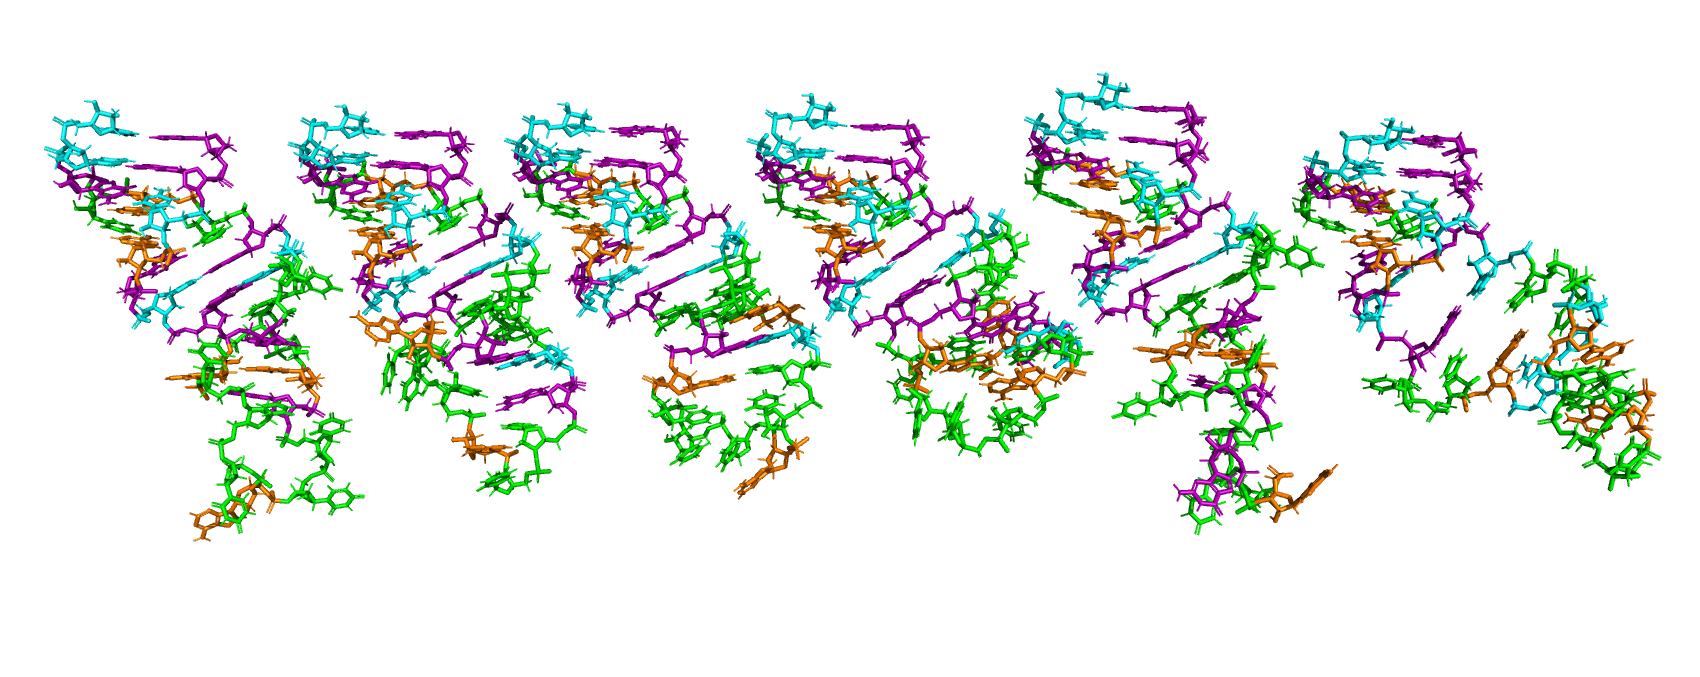
\includegraphics[width=\linewidth]{assets/RNAs.png}
    \caption[3D structures of the RNA motifs.]{3D structures of the RNA motifs. From left to right: the original RNA motif followed by the 5 mutants. Colors represent the nucleotidic bases: orange is Adenine, purple is Guanine, cyan is Cytosine and green is Uracil. Visualized through \href{https://pymol.org/2/}{\texttt{Pymol}}.}
    \label{fig:RNAs}
\end{figure}

With the 3D structures of the RNA motifs, the next step is to prepare the protein-RNA docking simulations.

\subsection{Protein-RNA docking simulations with \texttt{LightDock}}

For the protein-RNA docking simulations, the \texttt{LightDock} \cite{jimenez_garcia_2017} docking software was chosen. The main reasons are the simplicity of \texttt{LightDock}, the quality of the documentation and that the software is written in \texttt{Python}, which eases debugging steps in case of complications. Originally, \texttt{LightDock} was not meant for protein-RNA docking simulations. However, by means of some reasearch and auxiliary \texttt{Python} scripts, a simple and novel pipeline was designed which makes it possible to perform such docking simulations with \texttt{LightDock}. This pipeline takes inspiration on the \href{https://lightdock.org/tutorials/0.9.3/dna_docking}{protein-DNA docking example tutorial from the \texttt{LightDock} documentation}.

\subsubsection{Protein preparation}

First, MSI-1's RRM1 \texttt{.pdb} file needs to have their hydrogen atoms modified and relabeled so that they match the \texttt{AMBER94} force field, which is the parameter set that is going to be used in this docking simulation. To do so, the softwares \href{https://github.com/rlabduke/reduce}{\texttt{REDUCE}} and \href{https://github.com/haddocking/pdb-tools/}{\texttt{PDB-Tools}} \cite{rodrigues_2018} were employed.\\

In addition, the MSI-1's RRM1 \texttt{.pdb} file needed an additional motification related to the \texttt{AMBER94} force field: regular \texttt{.pdb} files employ the \texttt{HIS} identifier for the histidine aminoacid, which does not appear in the \texttt{AMBER94} force field. The reason behind this is that for the \texttt{AMBER94} force field, histidine can be one of 3 possible residues \cite{amber_histidine}:

\begin{enumerate}
    \item\texttt{HID}: histidine with a single hydrogen on the delta nitrogen
    \item\texttt{HIE}: histidine with a single hydrogen on the epsilon nitrogen
    \item\texttt{HIP}: histidine with hydrogens on both nitrogens (delta and epsilon). This histidine has a positive charge
\end{enumerate}

Therefore, one has to check which kind of histidine residue is present in the molecule, and change it for the corresponding \texttt{AMBER94}-compatible identifier. This can be done with a simple \texttt{Python} script called \texttt{fixHIS}, which is found in \textbf{\nameref{appendix_C}}.

\subsubsection{RNA preparation}

Similar to the protein, the RNA structures' \texttt{.pdb} file need to have their hydrogen atoms modified and relabeled. Again, the softwares \href{https://github.com/rlabduke/reduce}{\texttt{REDUCE}} and \href{https://github.com/haddocking/pdb-tools/}{\texttt{PDB-Tools}} \cite{rodrigues_2018} were employed.\\

In addition, \texttt{REDUCE} adds the 3' and 5' hydroxile groups to the RNA structures. These atoms aren't present in the \texttt{AMBER94} force field, therefore it is mandatory to remove them in order to avoid issues downstream. This can be done with a simple \texttt{Python} script called \texttt{removeEnds.py}, which is found in \textbf{\nameref{appendix_D}}.\\

Next, due to particularities of \texttt{REDUCE} for nucleic acids, it is necessary to rename and remove incompatible atom types present in the RNA structure. Again, this can be done with a simple \texttt{Python} script called \texttt{reduce\_to\_amber.py}, which is found in \textbf{\nameref{appendix_E}}. Note that the aforementioned \texttt{Python} script is an adaptation of the original version provided in the \href{https://lightdock.org/tutorials/0.9.3/dna_docking}{protein-DNA docking example tutorial from the \texttt{LightDock} documentation}.\\

Finally, in order to sucessfully run \texttt{LightDock}'s setup phase, it is mandatory to remove the \texttt{R} tags within the RNA structures. The \texttt{R} tags are important because they indicate which \texttt{AMBER94} parameters to use during the docking simulations, however one of \texttt{LightDock}'s dependencies in the setup phase (\href{http://prody.csb.pitt.edu/}{\texttt{ProDy}}) has conflicts with this notation. This removal can be done with a simple \texttt{Python} script called \texttt{manipulateRNA.py}, which is found in \textbf{\nameref{appendix_F}}.

\subsubsection{\texttt{LightDock} setup and simulation}

\texttt{LightDock}'s setup itself is simple, as it only consists of executing the setup script with the structures prepared in the previous steps, as shown in \textbf{Figure \ref{fig:lightdocksetup}}:

\begin{figure}[htbp!]
    \lstinputlisting[language=bash]{assets/lightdocksetup.sh}
    \caption{\texttt{LightDock} setup command.}
    \label{fig:lightdocksetup}
\end{figure}

The setup will generate, among other files, the simulation-ready structures\linebreak \texttt{lightdock\_protein.pdb} and \texttt{lightdock\_rna.pdb}. For the docking simulation to be successful, it is crucial to add the \texttt{R} tags within the \texttt{lightdock\_rna.pdb} RNA structure, which is basically reversing the tag removal process performed earlier. This can be achieved with a simple \texttt{Python} script called \texttt{manipulateRNAagain.py}, which is found in \textbf{\nameref{appendix_G}}.\\

\subsubsection{\texttt{LightDock} docking simulation, clustering and ranking}

If the previous steps executed without issues, it is possible to run \texttt{LightDock} as shown in \texttt{Figure \ref{fig:lightdockexec}}:

\begin{figure}[htbp!]
    \lstinputlisting[language=bash]{assets/lightdockexec.sh}
    \caption[\texttt{LightDock} execution command.]{\texttt{LightDock} execution command, using the \texttt{DNA} scoring function for nucleic acids and 4 processing cores.}
    \label{fig:lightdockexec}
\end{figure}

Once the simulation ends, and in order to be able to do the clustering and ranking step, it is mandatory to remove the \texttt{R} tags added to \texttt{lightdock\_rna.pdb} for the simulation step. For that, once again the script \texttt{manipulateRNA.py} shown in \textbf{\nameref{appendix_F}} is employed.\\

Next, the clustering and ranking can be performed in the same way as specified in the \href{https://lightdock.org/tutorials/0.9.3/dna_docking}{protein-DNA docking example tutorial from the \texttt{LightDock} documentation}. The \texttt{bash} script performing the ranking and clustering steps is shown in \textbf{\nameref{appendix_H}}.\\

The ranking will generate a \texttt{solutions.list} file where the different models generated by \texttt{LightDock} are scored. For this work, the top 10 best scoring models were taken.\\

The entire pipeline followed in this section has been implemented as a \texttt{bash} script called \texttt{run1.sh}, which is found in \textbf{\nameref{appendix_I}}. Given a\linebreak\texttt{target\_protein.pdb} file and a \texttt{ligand\_rna.pdb} file, \texttt{run1.sh} is executed as shown in \textbf{Figure \ref{fig:execrun1}}:

\begin{figure}[htbp!]
    \lstinputlisting[language=bash]{assets/run1exec.sh}
    \caption[Execution of the \texttt{run1.sh} script.]{Execution of the \texttt{run1.sh} script.}
    \label{fig:execrun1}
\end{figure}

A refined version of this pipeline has been contributed to the \href{https://lightdock.org/tutorials/0.9.3/index.html}{official \texttt{LightDock} tutorials section}. In said version, the \texttt{Python} scripts for file manipulation have been cleaned-up and applied to model the \href{https://www.rcsb.org/structure/1a1t}{1A1T protein-RNA complex}. This tutorial can be directly accessed \href{https://lightdock.org/tutorials/0.9.3/rna_docking}{here}.

% Las siguientes subsecciones son la liada parda que aún he de arreglar
\subsection{Fatty acid-protein docking simulations}
\subsection{Fatty acid-protein-RNA docking simulations}
